\documentclass[conference]{IEEEtran}
\usepackage{cite}
\usepackage{amsmath,amssymb,amsfonts}
\usepackage{algorithmic}
\usepackage{graphicx}
\usepackage{textcomp}
\usepackage{xcolor}
\usepackage{hyperref}
\usepackage{tabularx}

% COMMANDS
\newcommand{\R}{\mathbb{R}}
\newcommand{\fig}[1]{\textit{Figure \ref{1}}}
\newcommand{\eq}[1]{\textit{Equation \ref{1}}}

\begin{document}

\title{Applied AI in Biomedicine - Workshop Report}

% AUTHORS
\author{
    Alberto Rota
    \IEEEauthorblockA{ \\
    \textit{Person Code: 10615751}\\
    \textit{Student Number: 964662} \\
    \href{mailto:alberto2.rota@mail.polimi.it}{alberto2.rota@mail.polimi.it}}\\
\and
    Gabriele Santicchi 
    \IEEEauthorblockA{ \\
    \textit{Person Code: 10579046}\\
    \textit{Student Number: 969088}  \\
    \href{mailto:gabriele.santicchi@mail.polimi.it}{gabriele.santicchi@mail.polimi.it}}
    }
\maketitle

\section{Context}
    The goal of this project is to build a classification model that
    properly annotates each peaks as Normal, PAC (supraventricular
    beats) or PVC (ventricular beats). The available dataset is
    composed of 2-lead ECG signal and R peaks position of 105 patient 
    recordings. 

\section{Introduction}
    Electrocardiogram (ECG) signals records the electrical activity of
    the human hearts and consist of several waveforms (P, QRS, and T).
    The duration and shape of each waveform and the distances between
    different peaks are used to diagnose cardiovascular heart diseases
    (CVD). Premature atrial contractions (PAC) and premature
    ventricular contractions (PVC) are among the most common forms of
    arrhythmias; the first results from premature electrical
    activation originating in the atria of the heart, while the second
    one is caused by a premature electrical activation originating in
    the ventricles. As the presence of frequent PACs and PVCs are
    associated with a higher risk of unfavorable prognosis[1][2], the
    accurate recognition of these abnormal beats is strictly required.
    The aim of the this work is to design a deep-learning ensemble
    model that properly classifies all the peaks in a recording,
    without requiring the extraction of ECG features. The
    History-Time-Frequency Classifier analyzes each samples in both
    the time and frequency domain, and take as input also the labels
    assigned to the previous two samples. The miss-classification
    error on the test set was around 3\%, highlighting the potential
    of our classifier. 

\subsection{Dataset}
    The dataset consists of ECGs recorded from 105 patients
\section{Data Preprocessing}
The available raw dataset undergoes a pre-processing phase necessary for the
optimal interfacing between the data and the model.
\subsection{Exploratory Data Analysis}

\subsection{Signal Windowing}
The heartbeat-by-heartbeat classification that the model performs implies the
necessity of splitting the 30 minutes recording of each patient in windows, each
one to be processed separately by the network:
choosing the proper width and the optimal windowing approach is key in
obtaining the best model performance. Three different approaches have been taken
into consideration when splitting the windows, which are graphically compared in
\fig{fig:windows}.
\begin{figure}
    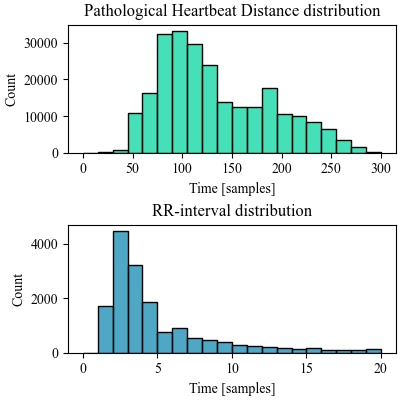
\includegraphics[width=\linewidth]{img/histograms.jpg}
    \label{fig:windows}
\end{figure}


\subsection{Class imbalance}

\section{The H.T.F. Model}
1. Parlare del class imbalance? Undersampling? 2. Mettere il graphviz
del modello? 
\subsection{H as History}
During a first inspection phase, an analysis on the distribution of
pathological beats has been performed. In fig. 1a, the histogram
reports the abnormal interpeak distances computed over all the
recordings, confirming that PACs and PVCs often occurs in repeated
patterns[3][4]. For these reasons, the involvement of the labels
assigned to the previous peak could help in predicting more precisely
the current peak. Considering the interpeak distances distributions,
in this classifier the two previous labels has been added as further
inputs of the ensemble model

\subsection{T as Time}
\subsection{F as Frequency}
The last branch of this model consists in a frequency-domain
classifier by a proper Fourier Transformation of the inputs. In order
to apply the Fourier Transform, the stationarity hypothesis has been
assumed for each window. This is not an heavy assumption, since the
inputs length is very short and most part of the window consists in
the peak recorded. The classifier consist of multiple
CNN-ReLU-MaxPooling stacks. A low filter size has been chosen to get
useful features in afew amount of samples at a time. After the
application of the FFT on the input signal, the output of the CNN
layer is concatenated with the two history-labels as in the time
model. Finally, a dense layer with a softmax AF provides the
probability assigned to the three labels. 

\section{Results}

\section{Discussion}

\section{Conclusions}

\end{document}